\section{Charaterization}
    %%%%%%%%%%%%%%%%%%%%%%%%%%%%%%%%%%%%%
	%%  Slide 1: <> %%
	%%%%%%%%%%%%%%%%%%%%%%%%%%%%%%%%%%%%%
    \begin{frame}
        \frametitle{Threshold and noise}
        The lower the threshold, the lower the minium detectable signal, allowing for thinner detector (Q$_{MIP}\propto$d). \\
        \medskip
        The threshold and the noise are \textbf{strictly} related with the \textbf{FE} status\\
        \medskip
        What determins the minimum stable threshold?
        \begin{itemize}
            \item the \textbf{ENC} 
            \item the \textbf{threshold dispersion} 
        \end{itemize}
        \medskip
        Numeri attesi da simulazione with optimal FE settings
        \begin{center}
        \begin{beamercolorbox}[rounded=true, center]{palette light primary}
            Noise \hspace*{1.2cm} Threshold \hspace*{1.2cm} Threshold dispersion
        \end{beamercolorbox}
        \begin{beamercolorbox}[rounded=true, center]{palette titleframe}
            \hspace*{-2.4cm} $\sim$\SI{9}{\elementarycharge}$^-$ \hspace*{1.4cm} $\sim$\SI{270}{\elementarycharge}$^-$ \hspace*{1.2cm} $\sim$\SI{30}{\elementarycharge}$^-$
        \end{beamercolorbox}
    \end{center}
    \end{frame}


    %%%%%%%%%%%%%%%%%%%%%%%%%%%%%%%%%%%%%
	%%  Slide 1: <Scurve> %%
	%%%%%%%%%%%%%%%%%%%%%%%%%%%%%%%%%%%%%
    \begin{frame}
        \frametitle{Threshold and noise: how to measure them?}
        \begin{itemize}
            \item\textbf{Iinternal injection circuit}: allows sending a voltage step on an injecting capacitance C$_{inj}$ at the FE input
        \end{itemize}
        \bigskip
        \begin{columns}
            \column{0.45\textwidth}  
                Efficiency vs injected charge at fix threshold
                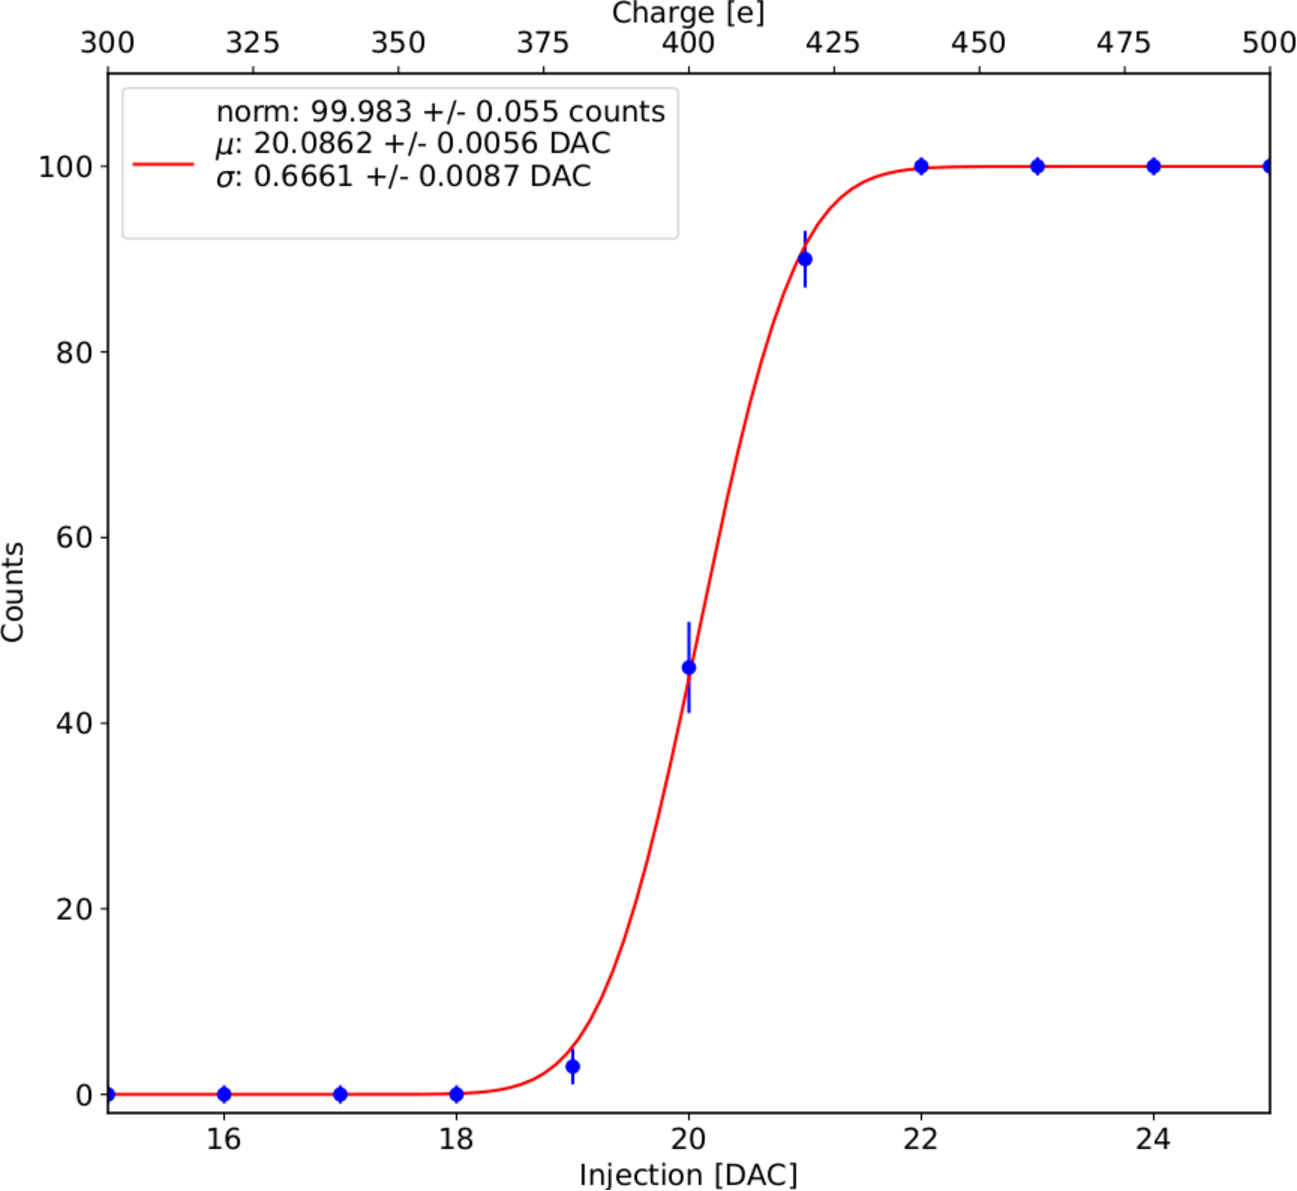
\includegraphics[width=1.1\linewidth]{figures/charaterization/scurve.pdf}
            \column{0.55\textwidth} 
                By design:
                \begin{beamercolorbox}[ rounded=true, center]{lightbluebox}
                    C$_{inj}$=\SI{230}{fF} $\rightarrow$ Q$_{inj}$=\SI{20}{\elementarycharge}$^-$/DAC
                \end{beamercolorbox}
                \\
                \bigskip
                Assuming a gaussian noise:
                \begin{itemize}
                    \item the threshold is the 50\%
                    \item the noise is 1/slope 
                \end{itemize}
                \medskip
                Analitical parametrization of the curve with the $error\,function$
                %\begin{equation*}
                %    \tiny
                %    f(x, \mu, \sigma) = \frac{1}{2} \; \left(1\,+\,erf\left(\frac{x-\mu}{\sigma \sqrt{2}}\right)\right)
                %    \label{eq:fit_scurve}
                %\end{equation*}
        \end{columns}
    \end{frame}

    %%%%%%%%%%%%%%%%%%%%%%%%%%%%%%%%%%%%%%%%
    %%  Slide 4: <ToT vs charge>  %%
    %%%%%%%%%%%%%%%%%%%%%%%%%%%%%%%%%%%%%%%%
    \begin{frame}
        \frametitle{Calibration of the signal}
        Q$_{inj}$ depends on the C$_{inj}$, different for each pixel.     
        \bigskip
        How convert the DAC units in electrons collected in the sensor?\\
        \begin{itemize}
            \item linearity of the output signal 
            \item need of a reference, radioactive source
            \item ATTENZIONE A COME CITI LA LINEARITÀ CHE È MISLEADING
            \item Formula per la calibrazione. 
        \end{itemize}
        \bigskip
        \begin{beamercolorbox}[sep=0em,wd=0.85\textwidth,ht=1.5ex, dp=0.1ex, rounded=true, center]{lightbluebox}
            Fe$^{55}$ $\rightarrow$ Mn$^{55}$ + K$_\alpha$ (\SI{5.9}{keV}) or K$_\beta$ (\SI{6.5}{keV})
        \end{beamercolorbox}
        \begin{tikzpicture}[overlay]
            \draw[decorate,decoration={brace}]
                (3.5,0) -- (5.5,0);
        \end{tikzpicture}
        \begin{columns}
            \column{0.2\textwidth}             
            \column{0.8\textwidth}             
            \begin{itemize}
                \item $\lambda$=\SI{29}{\um}$\rightarrow$ P$_{abs}$=, photo-electric effect
                \item $w_i$=\SI{3.6}{eV} in Si @ \SI{300}{\kelvin}$\rightarrow$ \SI{1616}{\elementarycharge}$^-$
            \end{itemize}
        \end{columns}
    \end{frame}  


    %%%%%%%%%%%%%%%%%%%%%%%%%%%%%%%%%%%%%%%%
    %%  Slide 3: <ToT linearity>  %%
    %%%%%%%%%%%%%%%%%%%%%%%%%%%%%%%%%%%%%%%%
    \begin{frame}
        \frametitle{ToT linearity}
        \begin{itemize}
            \item linearity is due to the \textbf{PMOS} reset circuit of the amplifier which guaranties that the discharge of the preamplifier is costant in time. Then the ToT is completely correlated with the pulse amplitude 
            \item ToT is saved as a 6-bits variable and can vary in range 0-63
            \item calibrated with the injection
        \end{itemize}
        \medskip
        \medskip
        \medskip
        \begin{columns}
            \column{0.5\textwidth}  
                \includegraphics[width=.8\linewidth]{figures/Monopix1/pulse_60to10.png}
            \column{0.5\textwidth}
                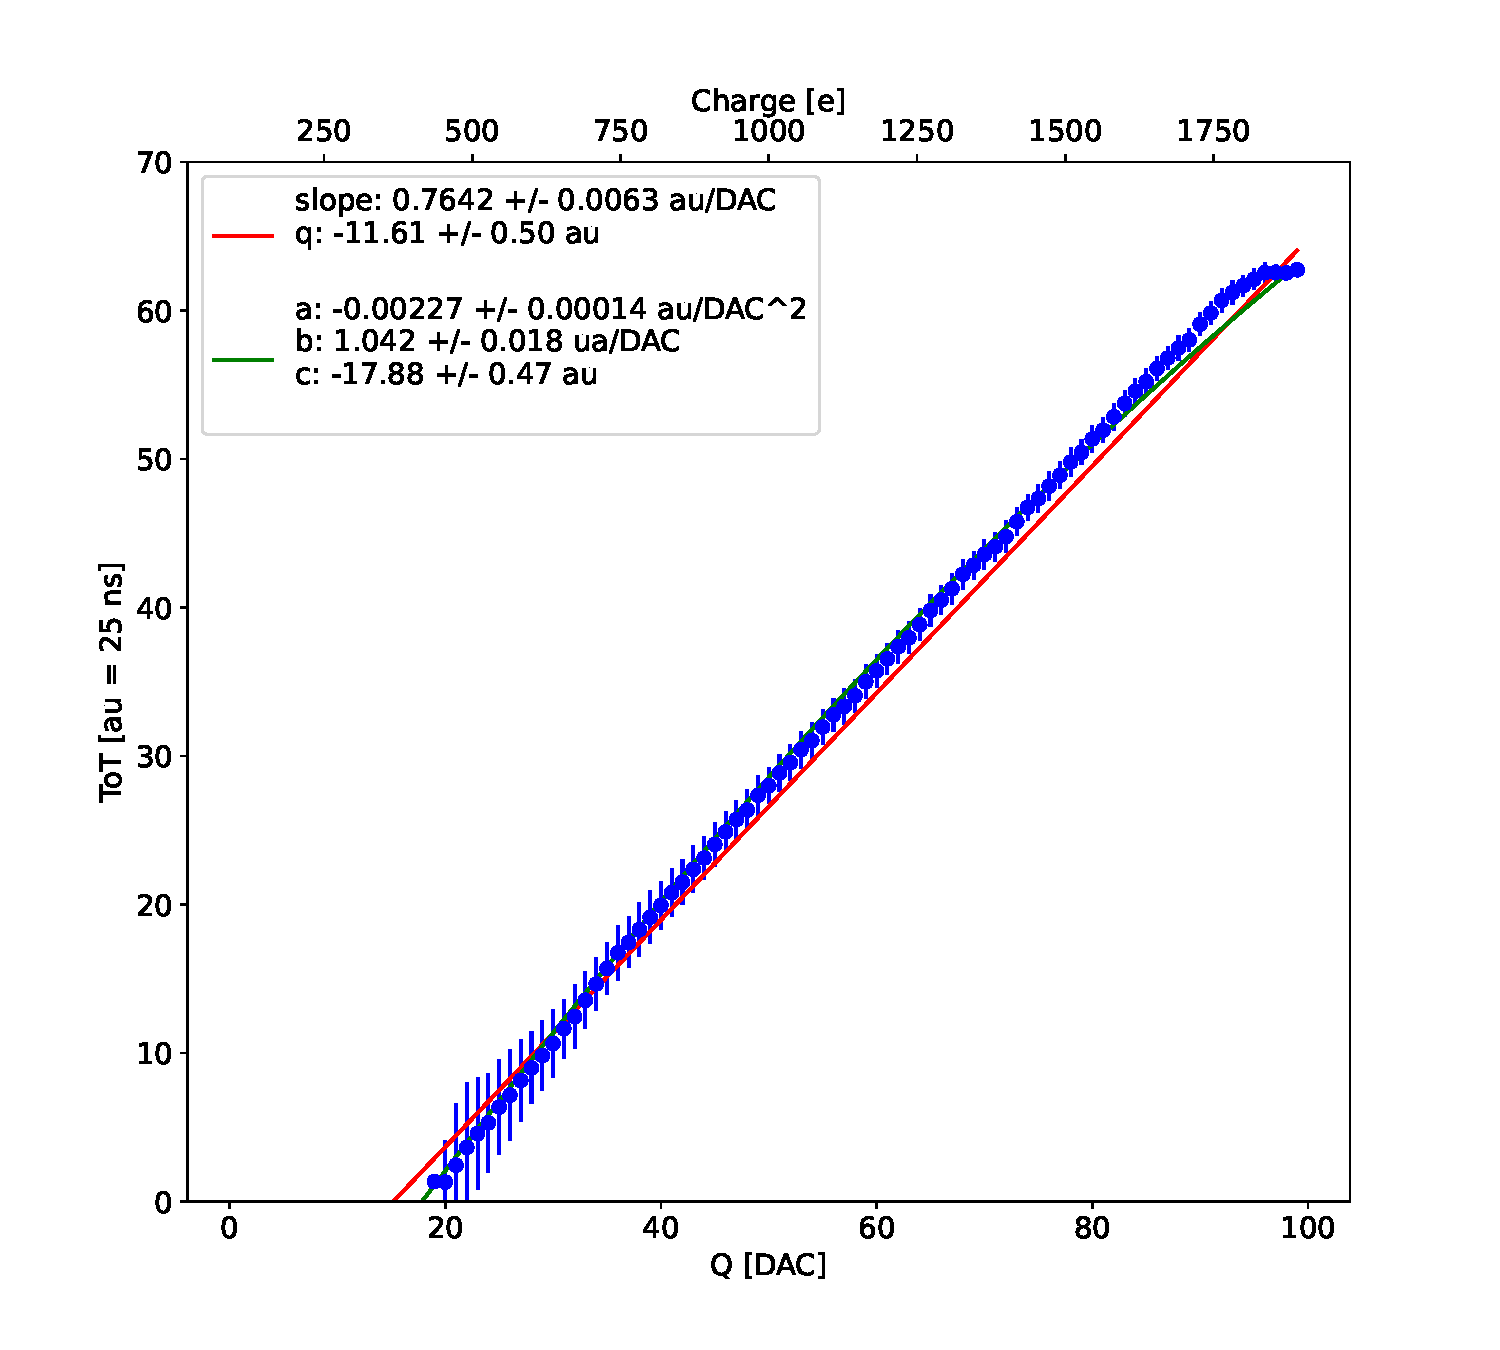
\includegraphics[width=.8\linewidth]{figures/charaterization/ToT_injection.pdf} 
        \end{columns}
    \end{frame}    

    %%%%%%%%%%%%%%%%%%%%%%%%%%%%%%%%%%%%%%%%
    %%  Slide 4: <ToT calibration>  %%
    %%%%%%%%%%%%%%%%%%%%%%%%%%%%%%%%%%%%%%%%
    \begin{frame}
        \frametitle{ToT absolute calibration: Fe$^{55} \rightarrow$ Mn$^{55}$ K$_{\alpha}$}
        Long tail on the left corresponds to partial absorption of the charge produced by the photo-electron
        \begin{columns}
            \column{0.5\textwidth}                  
                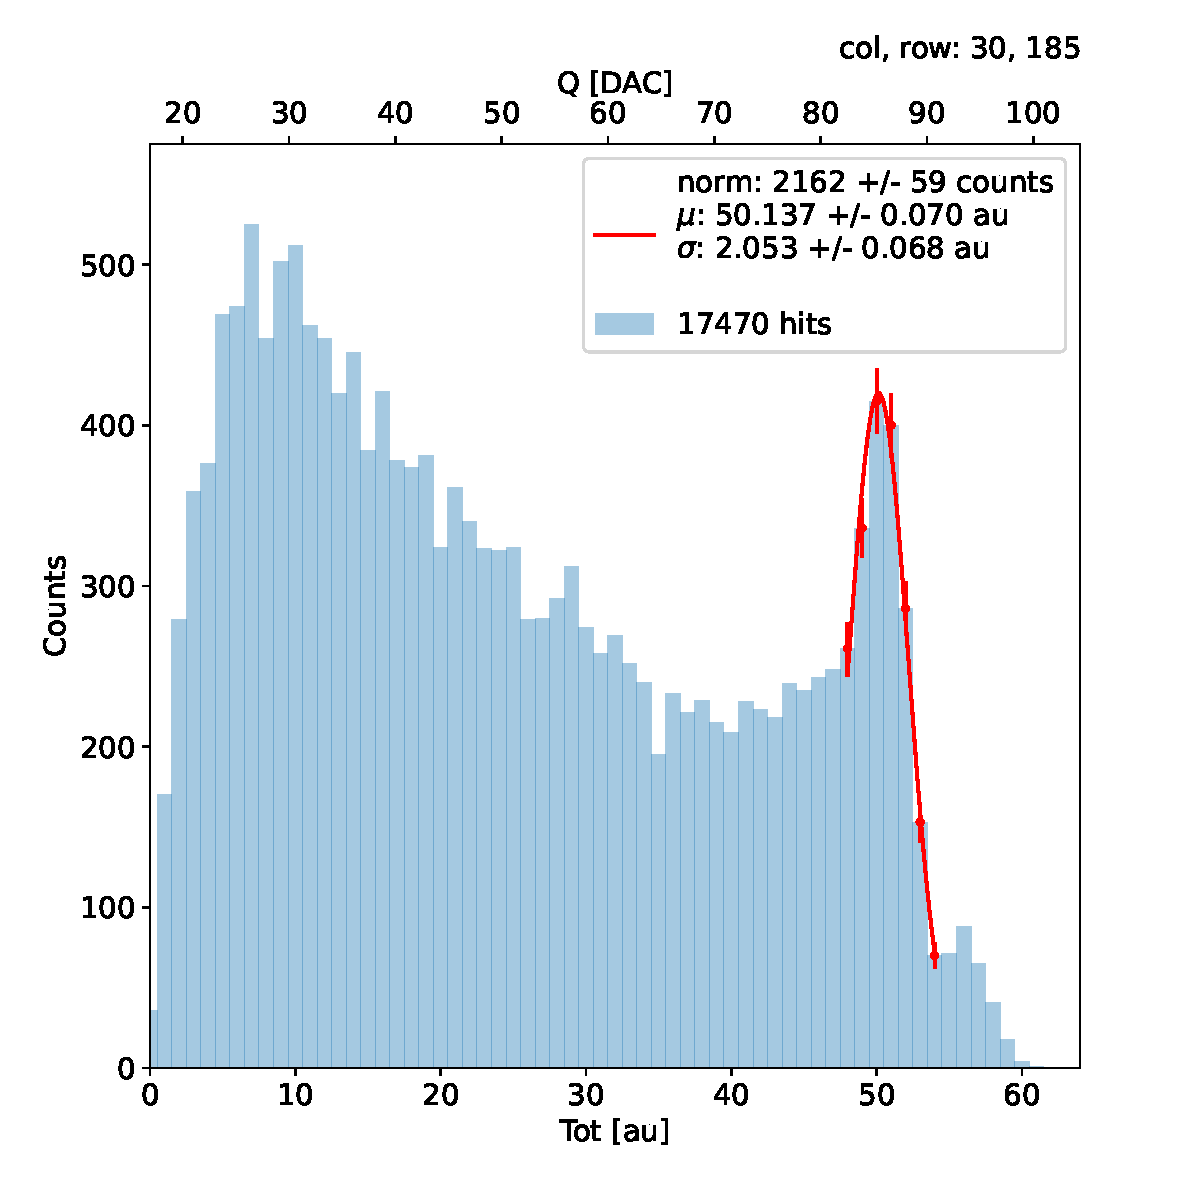
\includegraphics[width=1.25\linewidth]{figures/charaterization/fit_gauss_r185.pdf}
            \column{0.5\textwidth}    
            \begin{enumerate}
                \item Fit with a gaussian to find the peak position in the spectrum
                \item Conversion from ToT in DAC (using the line parameters)
                \item Peak value in DAC fixed to be equal to \SI{1616}{\elementarycharge}$^-$
            \end{enumerate} 
        \end{columns}
    \end{frame}     


    %%%%%%%%%%%%%%%%%%%%%%%%%%%%%%%%%%%%%%%%
    %%  Slide 4: <ToT calibration>  %%
    %%%%%%%%%%%%%%%%%%%%%%%%%%%%%%%%%%%%%%%%
    \begin{frame}
        \frametitle{Different collection properties}
        2 different \textbf{dose profile} in the sensor: Reduced Deep P-Well (RDPW) and Full Deep P-Well (FDPW)

        \begin{itemize}
            \item Different charge collection efficiency due to the deep p-well structure within the sensor
        \end{itemize}
        \begin{columns}
            \column{0.5\textwidth}                  
                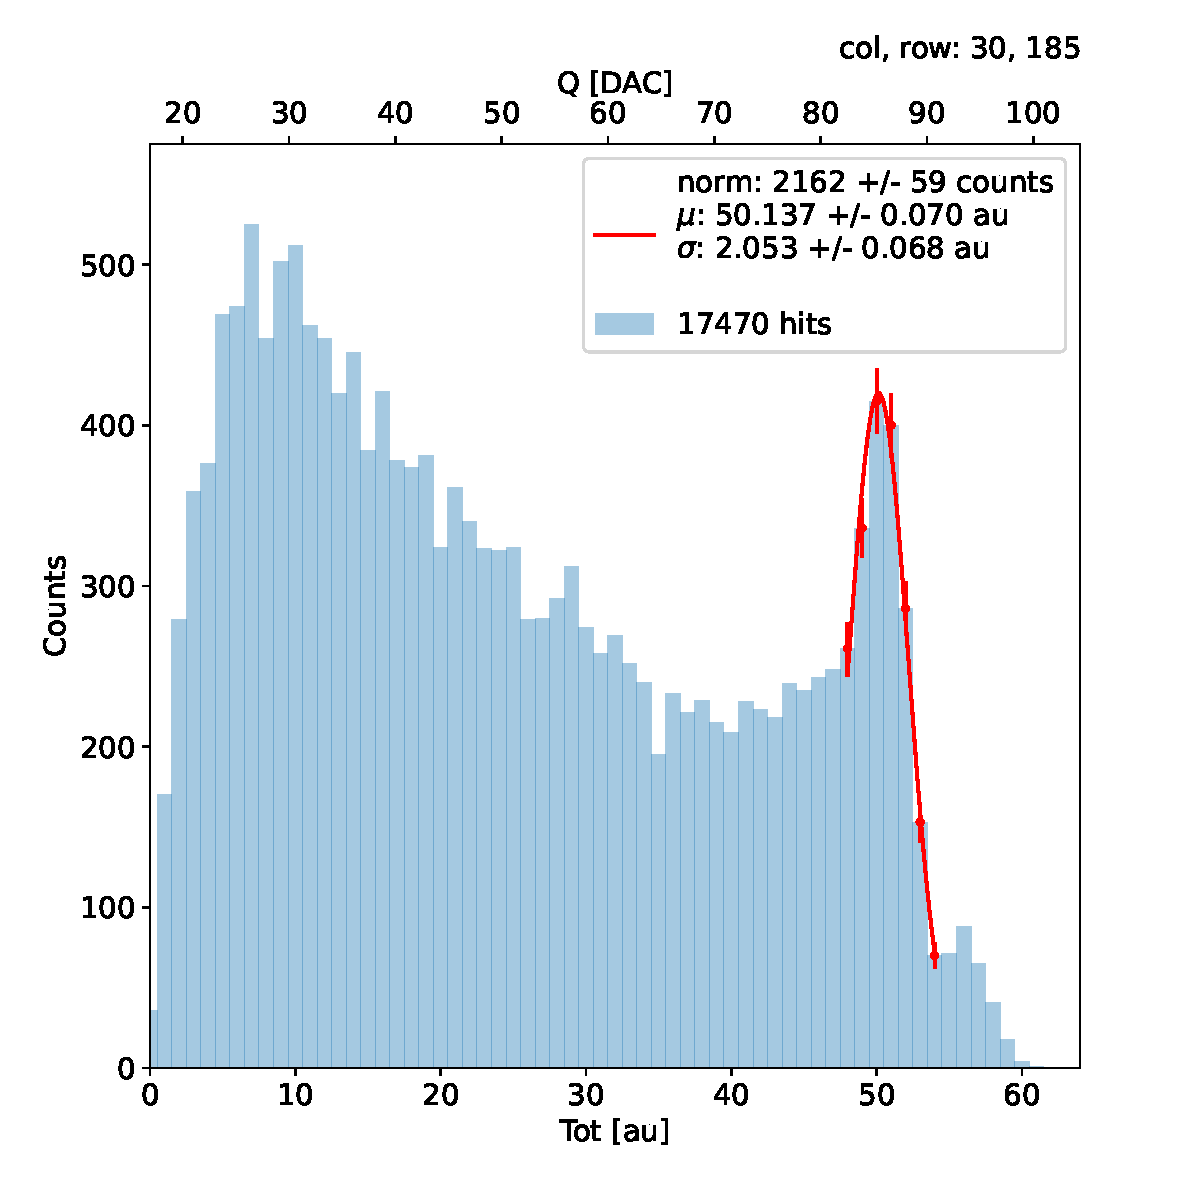
\includegraphics[width=1.1\linewidth]{figures/charaterization/fit_gauss_r185.pdf}
                \centering Full deep p-well
            \column{0.5\textwidth}    
                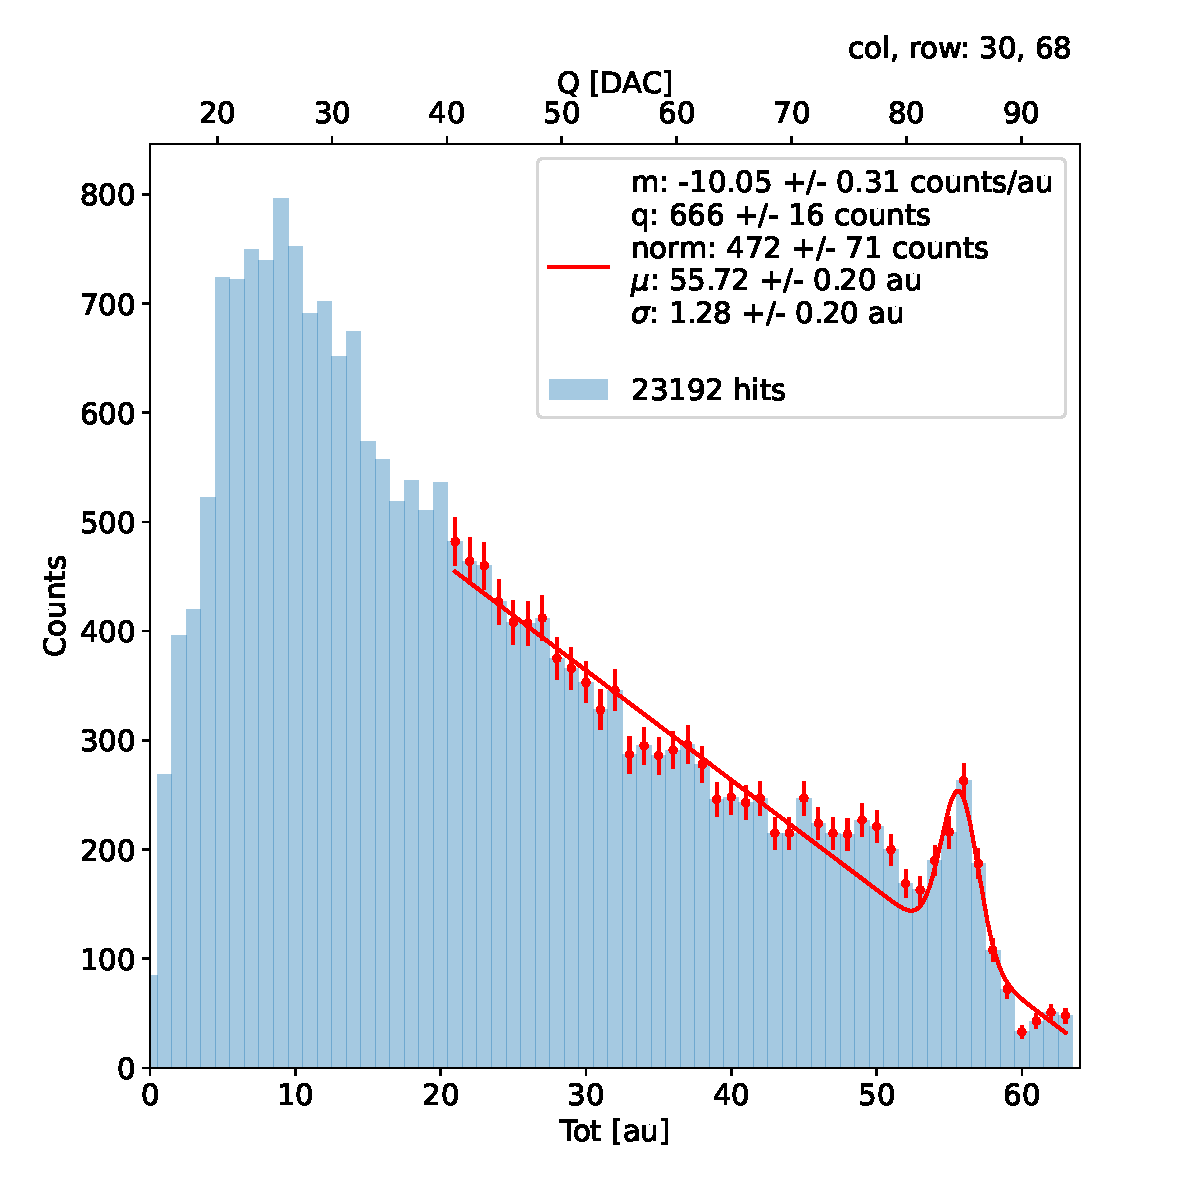
\includegraphics[width=1.1\linewidth]{figures/charaterization/fit_line_gauss_r69.pdf}
                \centering Partial deep p-well
        \end{columns}
    \end{frame}


    %%%%%%%%%%%%%%%%%%%%%%%%%%%%%%%%%%%%%%%%
    %%  Slide 4: <ToT calibration>  %%
    %%%%%%%%%%%%%%%%%%%%%%%%%%%%%%%%%%%%%%%%
    \begin{frame}
        \frametitle{Calibration results}
        \begin{columns}
            \column{0.5\textwidth} 
            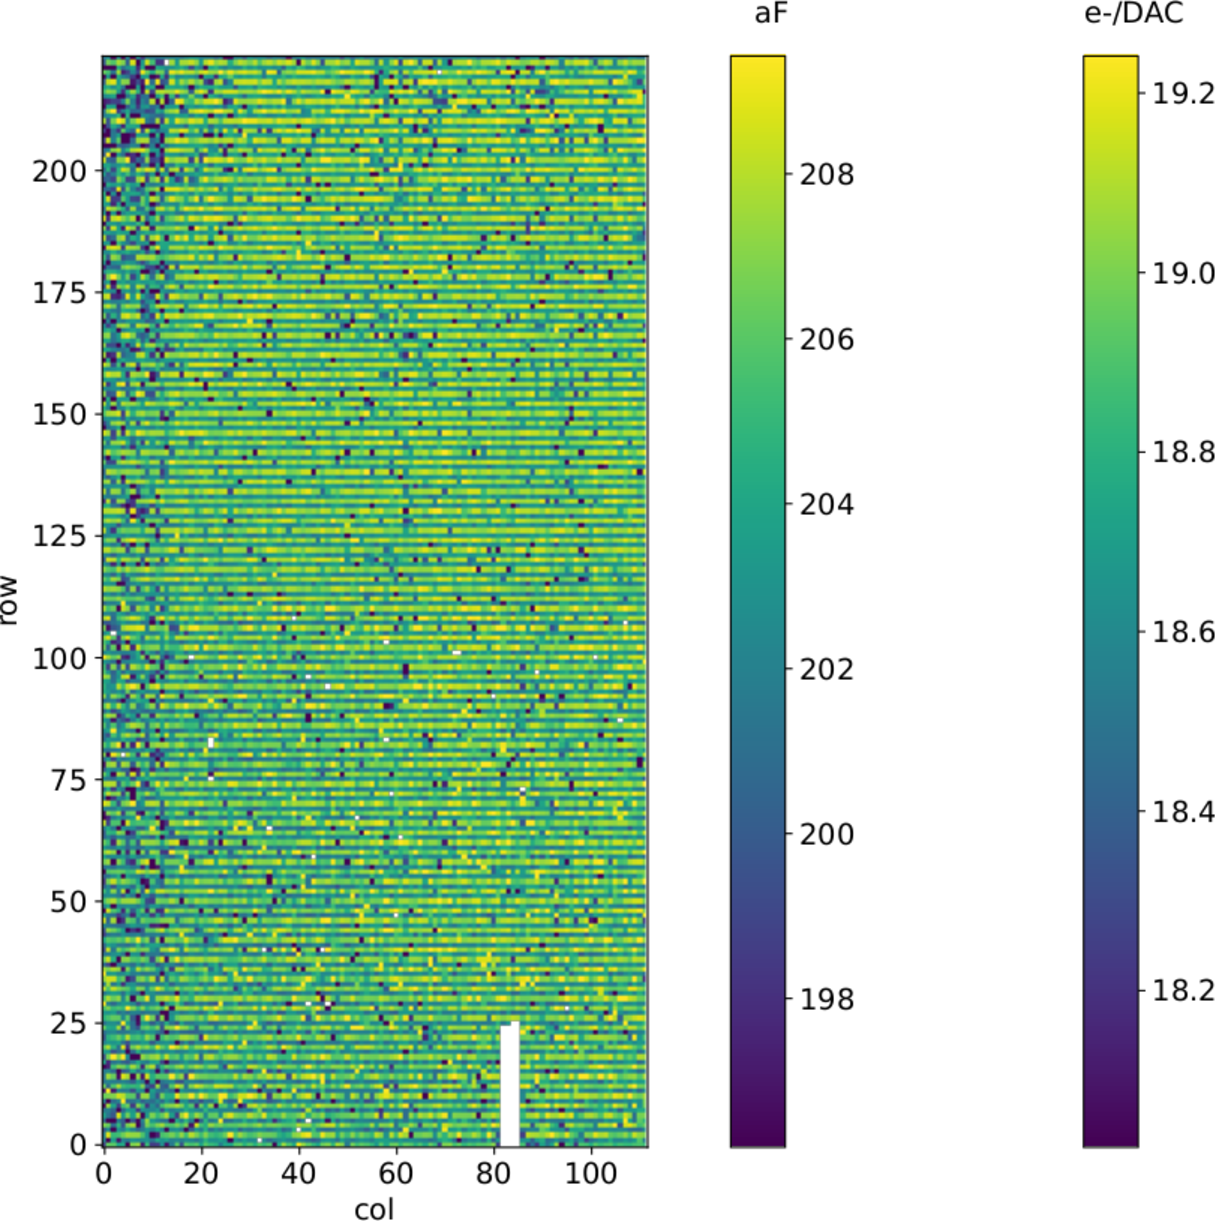
\includegraphics[width=1.1\linewidth]{figures/charaterization/conversion_factor_map.pdf}
            \column{0.5\textwidth} 
            \begin{itemize}
                \item C$_{inj}$ is in range 180-200\si{fF} (exp. \SI{230}{fF})
                \item F is is range 16.5-18.5 (exp. \SI{20.2}{\elementarycharge/DAC}$^-$)
                \item structure on rows probably due to bias line differences in the injection circuit 
                \item applying the calibration the threshold and noise are respectively \SI{340}{\elementarycharge}$^-$ and \SI{10}{\elementarycharge}$^-$
            \end{itemize}
        \end{columns}
    \end{frame}


    %%%%%%%%%%%%%%%%%%%%%%%%%%%%%%%%%%%%%%%%
    %%  Slide 5: <ToT bias>  %%
    %%%%%%%%%%%%%%%%%%%%%%%%%%%%%%%%%%%%%%%%
    \begin{frame}
        \frametitle{Changing the bias}
        \begin{columns}
            \column{0.3\textwidth} 
                Acquisitions with:
                \begin{itemize}
                    \item Injection
                    \item Fe$^{55}$ source
                \end{itemize}
            \column{0.7\textwidth} 
                %Maximum bias suggested
                \begin{table}
                    \begin{center}
                    \scalebox{0.75}{
                    \begin{tabular}{| c |  c | c | c |}
                    \hline
                    & -\SI{6}{V} & -\SI{3}{V} & \SI{0}{V}\\
                    \hline
                    \hline
                    Threshold [DAC] & 20 $\pm$ 2 & 21 $\pm$ 2 & 24 $\pm$ 2\\
                    Noise [DAC] & 0.61 $\pm$ 0.08 & 0.62 $\pm$ 0.08 & 0.82 $\pm$ 0.1\\
                    \hline
                    \end{tabular}}
                    \end{center}
                \end{table}
        \end{columns}
        \begin{columns}
            \column{0.4\textwidth}          
            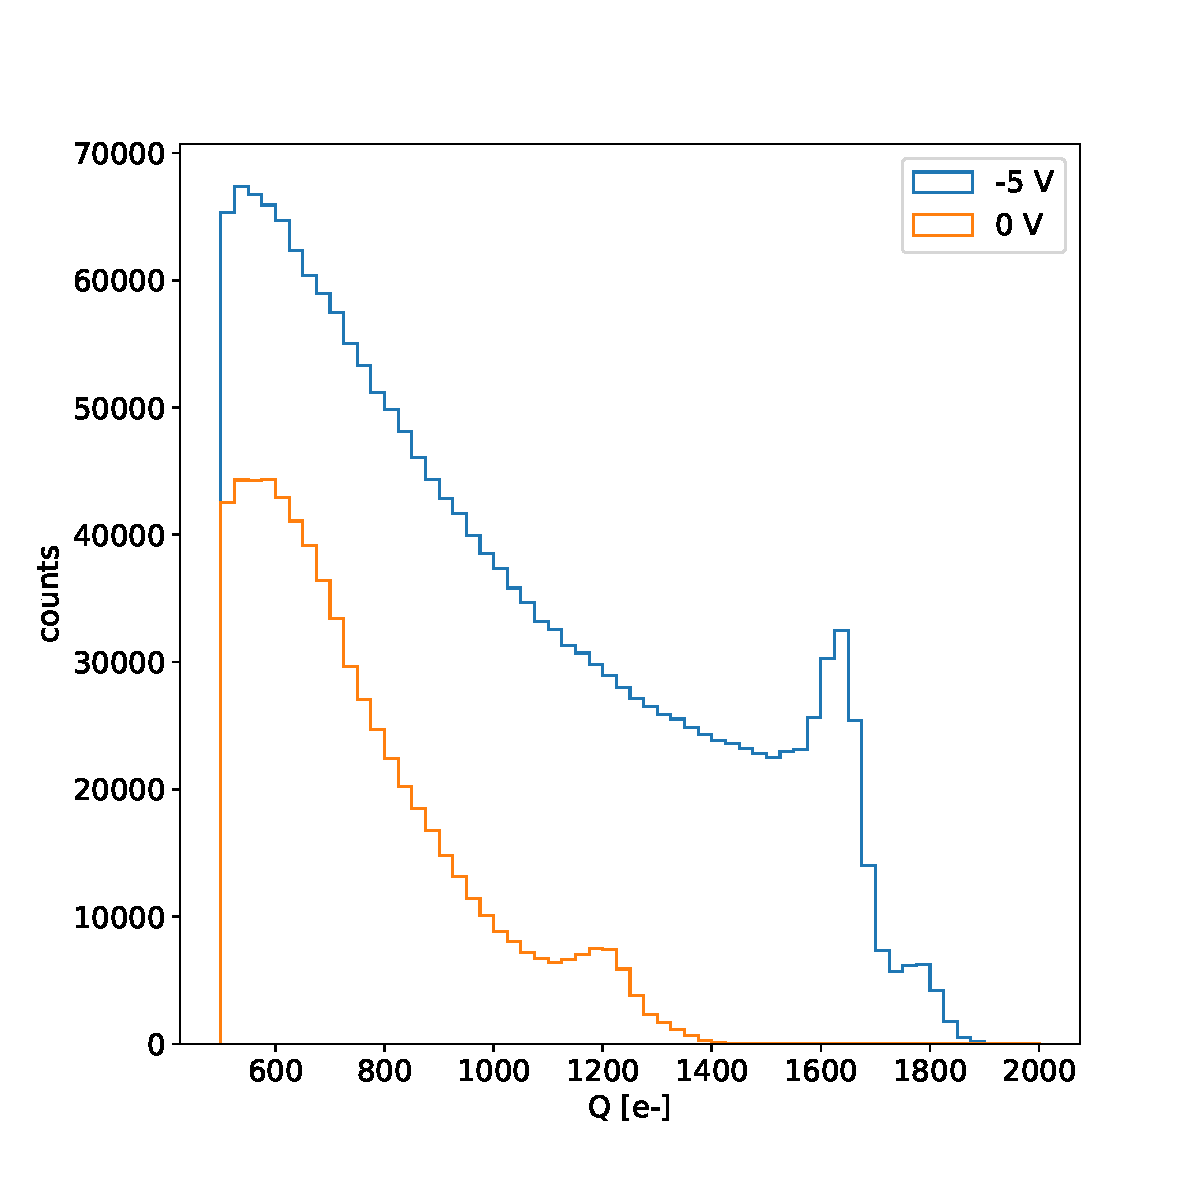
\includegraphics[width=1.2\linewidth]{figures/charaterization/Fe_spectrum_bias.pdf}
        \column{0.6\textwidth}
            Reducing the bias from -\SI{6}{V} to \SI{0}{V} reduction of the below quantity in the Fe$^{55}$ spectrum: 
            \begin{enumerate}
                \item ToT value of the peak $\sim$30\%
                \item N of events under the peak $\sim$60\%
                \item hit rate $\sim$60\%
            \end{enumerate}
            1 is due to the reduction in the gain, 2 and 3 are due to the decrease in the depletion thickness
          
        \end{columns}
    \end{frame}      


    %%%%%%%%%%%%%%%%%%%%%%%%%%%%%%%%%%%%%%%%
    %%  Slide 4: <Aquisitions with sources>  %%
    %%%%%%%%%%%%%%%%%%%%%%%%%%%%%%%%%%%%%%%%
    \begin{frame}
        \frametitle{Acquisition with sources: Fe$^{55}$, Sr$^{90}$, cosmic rays}
        \begin{columns}
            \column{0.35\textwidth} 
                \begin{table}
                    \tiny
                    \begin{center}
                    \begin{tabular}{|c | c |}
                    \hline
                    Source & Rate [\si{Hz}]\\
                    \hline
                    \hline
                    Fe$^{55}$ & 3.3 10$^3$\\
                    Sr$^{90}$ & \\
                    CR & \\
                    Noise &  \\
                    \hline
                    \end{tabular}
                    \end{center}
                \end{table}

            \column{0.65\textwidth} 
                \begin{itemize}
                    \item Fe$^{55}$ photon produces smaller clusters: pure charge sharing
                    \item Sr$^{90}$ and cosmic rays go across more pixels 
                \end{itemize}    
        \end{columns}
        \medskip
        \begin{columns}
            \column{0.5\textwidth} 
            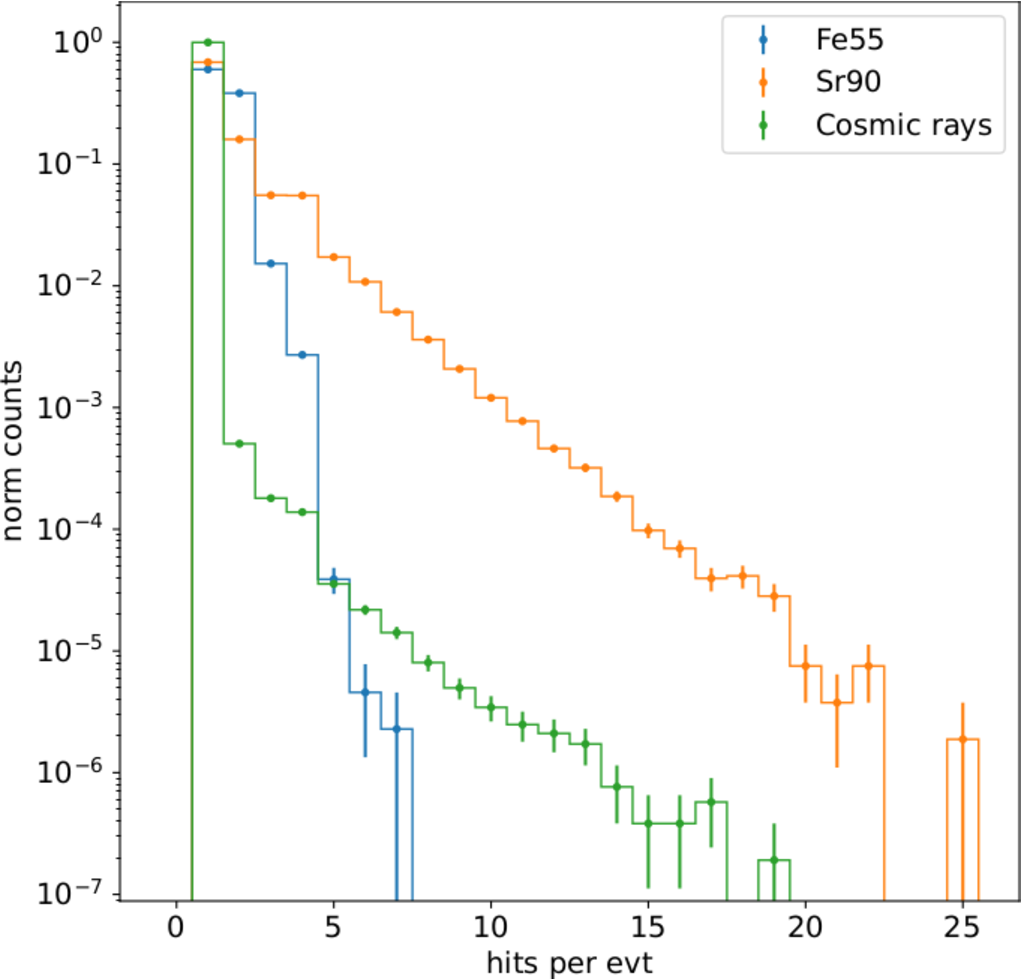
\includegraphics[width=1.\linewidth]{figures/charaterization/hits_per_evt.png}            
            \column{0.5\textwidth} 
            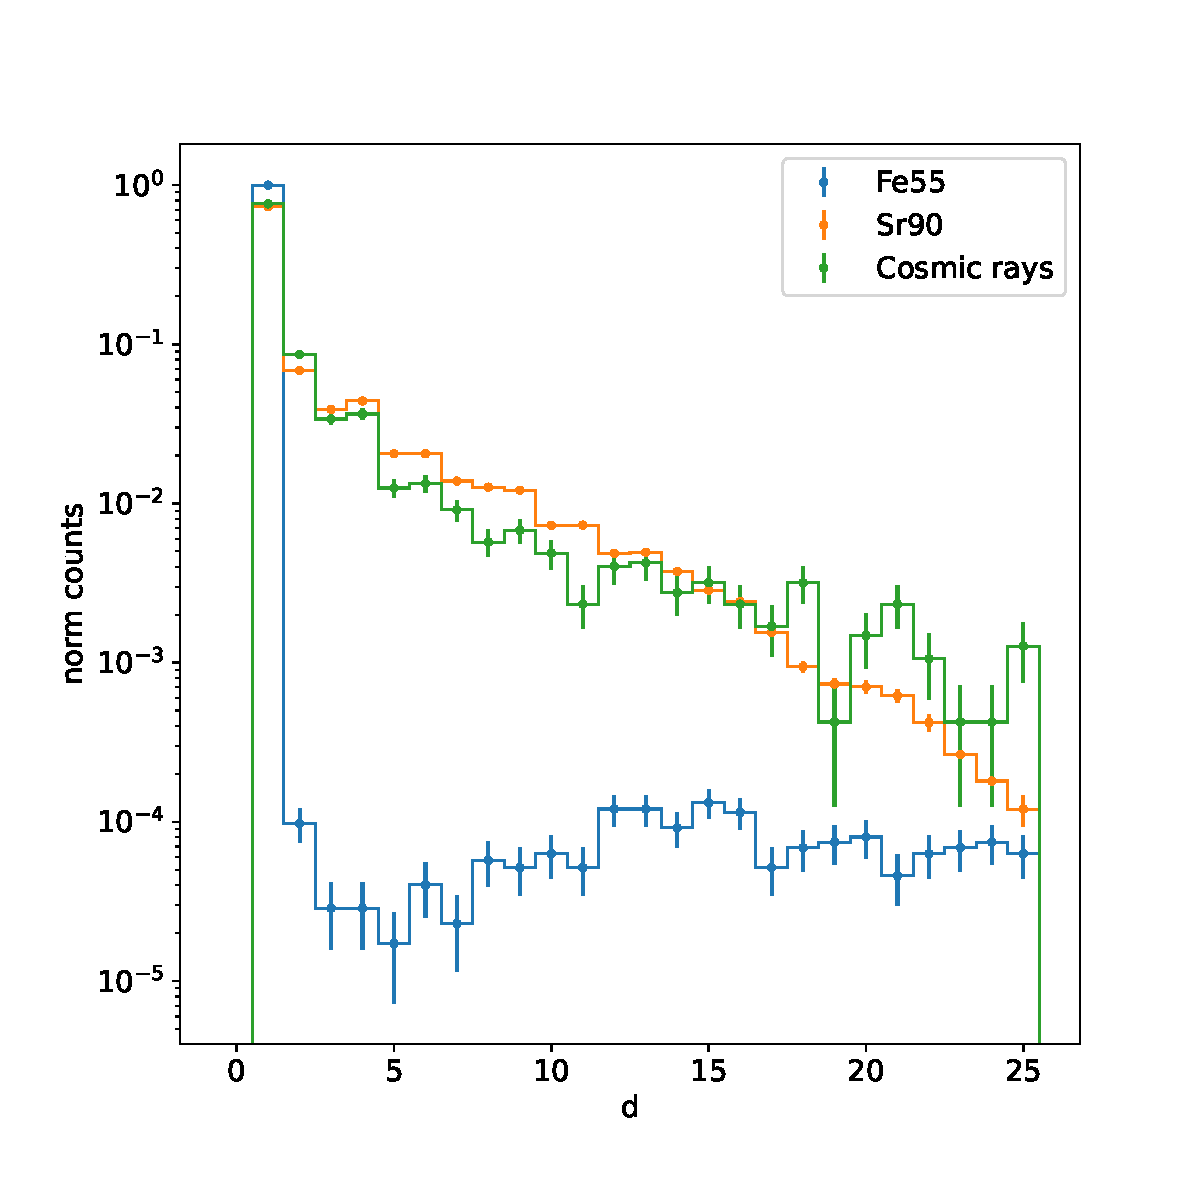
\includegraphics[width=1.\linewidth]{figures/charaterization/cluster_dimension.pdf}
        \end{columns}
    \end{frame}    


    %%%%%%%%%%%%%%%%%%%%%%%%%%%%%%%%%%%%%%%%
    %%  Slide 4: <Aquisitions with sources>  %%
    %%%%%%%%%%%%%%%%%%%%%%%%%%%%%%%%%%%%%%%%
    \begin{frame}
        \frametitle{Acquisition with Sr$^{90}$$\rightarrow$Y$^{90}$$\beta^-$$\rightarrow$Zr$^{90}$$\beta^-$}
        \begin{columns}
            \column{0.5\textwidth} 
                \begin{itemize}
                    \item Q released per pixel
                \end{itemize}
                \bigskip
                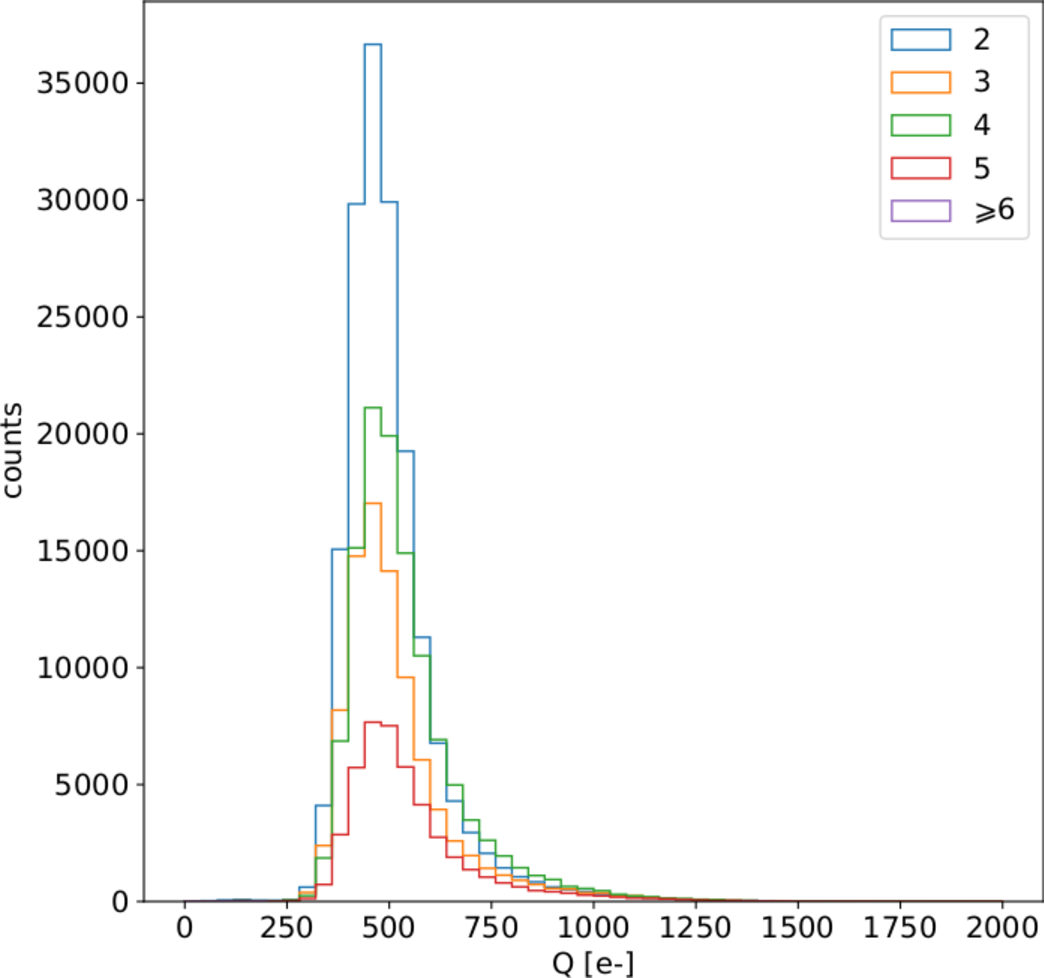
\includegraphics[width=1.1\linewidth]{figures/charaterization/Sr90_spectrum_per_pixel.pdf} 
            \column{0.5\textwidth} 
            E$_{e, max}$=\SI{546}{keV}, E$_{e, max}$=\SI{2.3}{MeV}
                \begin{figure}
                    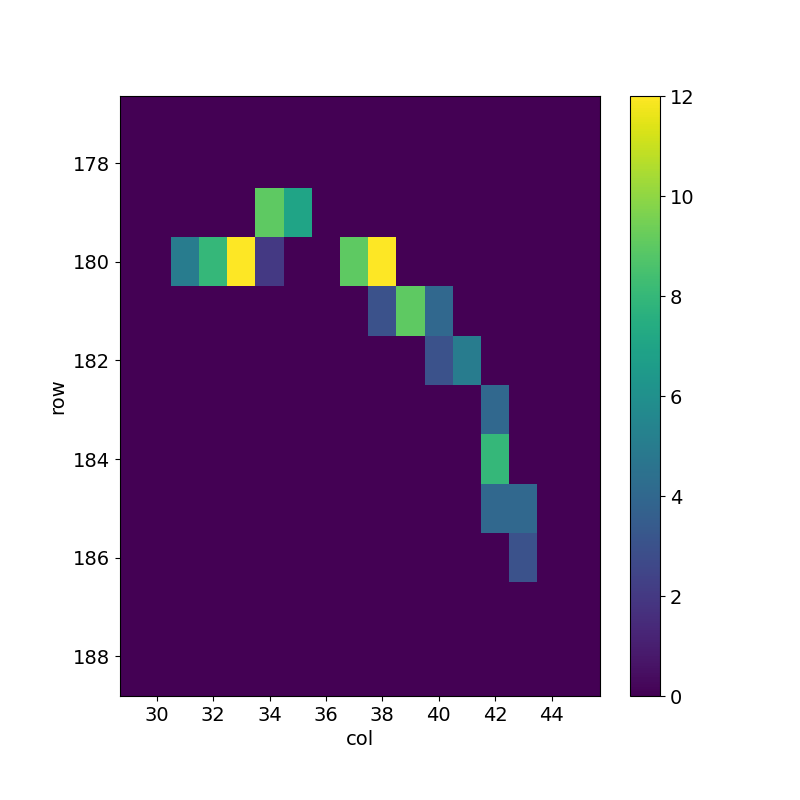
\includegraphics[width=.3\linewidth]{figures/charaterization/evts/Sr90/18b.png}
                    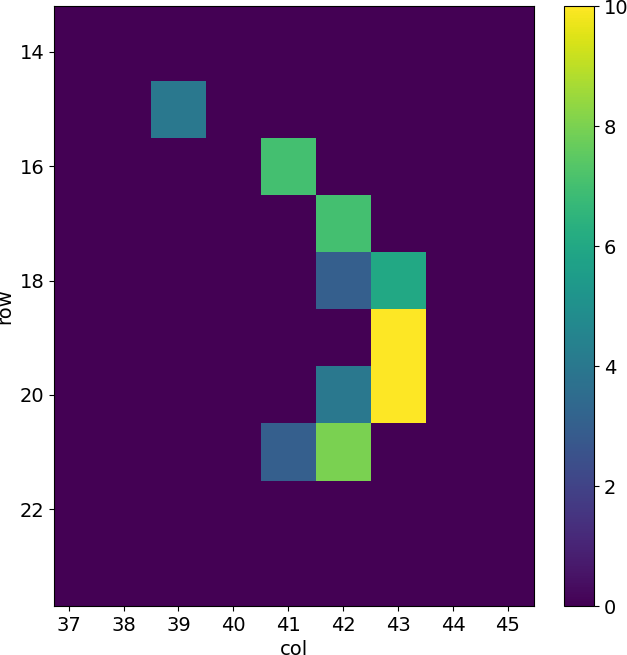
\includegraphics[width=.3\linewidth]{figures/charaterization/evts/Sr90/10b.png} 
                    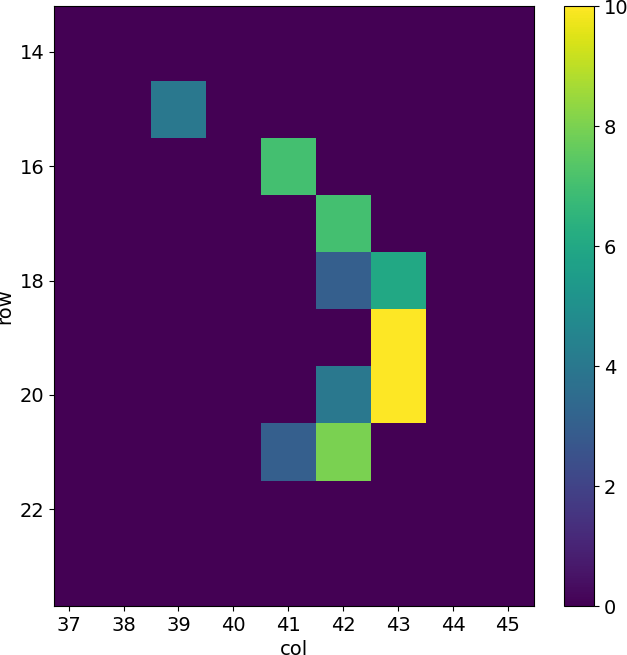
\includegraphics[width=.3\linewidth]{figures/charaterization/evts/Sr90/10b.png}
                \end{figure}
                \begin{itemize}
                    \item Q in cluster is proportional to the cluster size
                    \item due to large angle electrons
                    \item MPV $\sim$\SI{500}{\elementarycharge}$^-$
                    \item charge sharing between pixels 
                \end{itemize}
        \end{columns}
    \end{frame}    

    %%%%%%%%%%%%%%%%%%%%%%%%%%%%%%%%%%%%%%%%
    %%  Slide 4: <Aquisitions with sources>  %%
    %%%%%%%%%%%%%%%%%%%%%%%%%%%%%%%%%%%%%%%%
    \begin{frame}
        \frametitle{Acquisition with cosmic rays}
        \begin{columns}
            \column{0.5\textwidth} 
                \begin{itemize}
                    \item Q released per pixel
                \end{itemize}
                \bigskip
                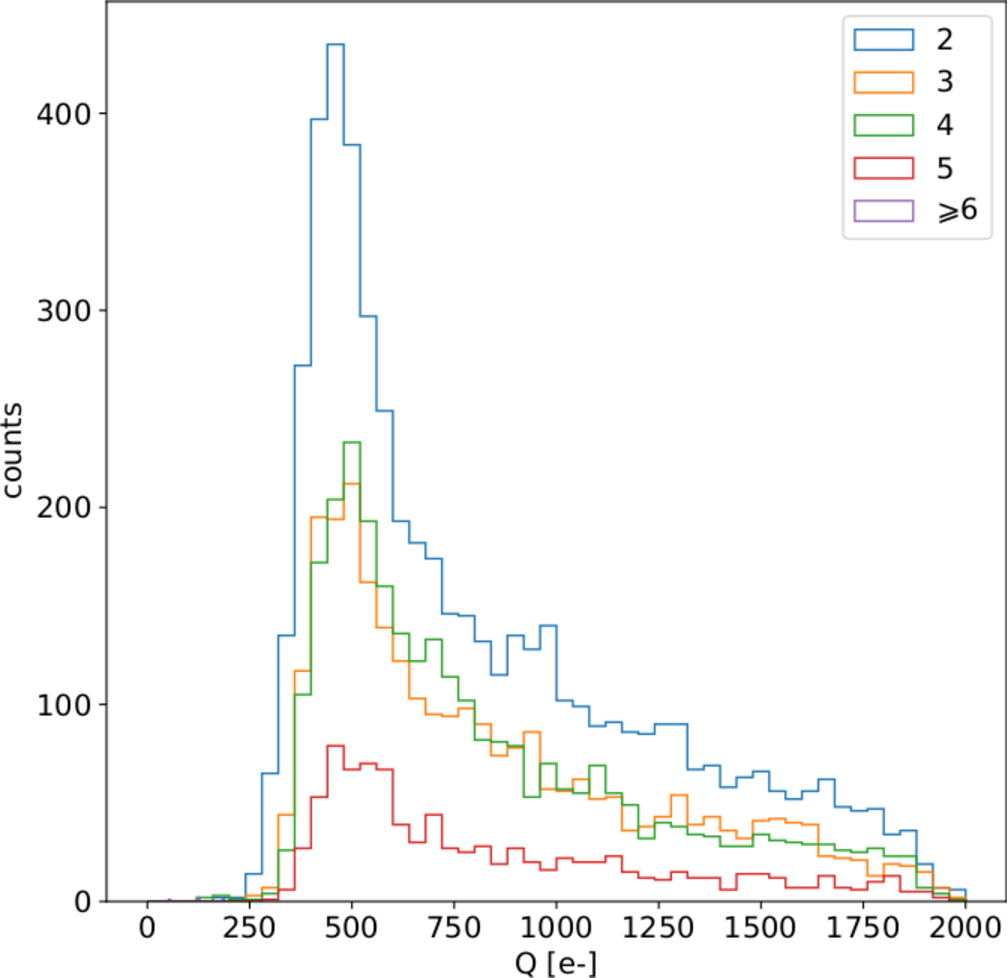
\includegraphics[width=1.1\linewidth]{figures/charaterization/cosmic_rays_spectrum_per_pixel.pdf} 
            \column{0.5\textwidth} 
                \begin{figure}
                    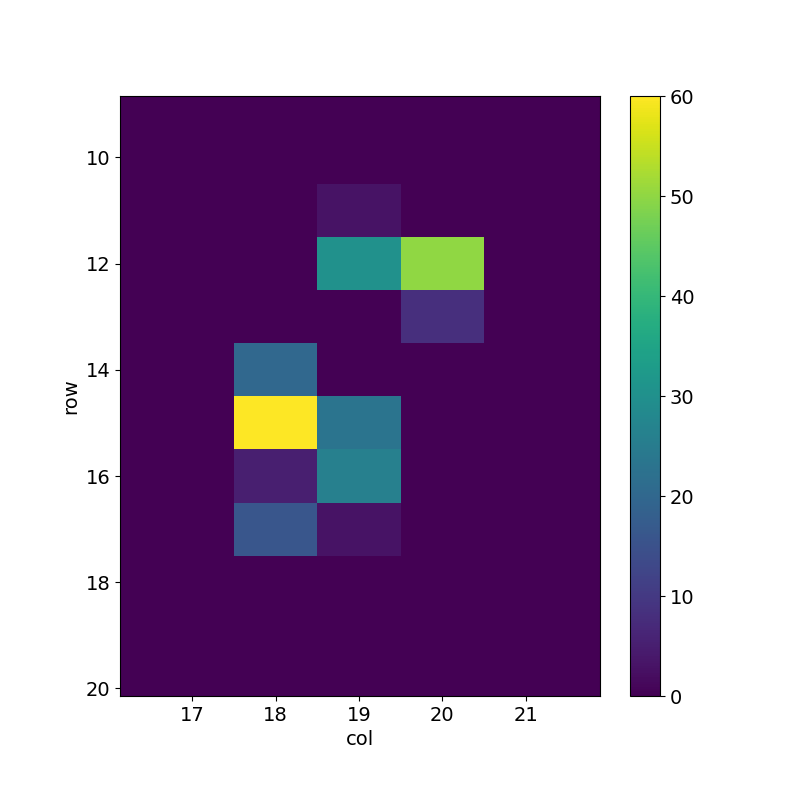
\includegraphics[width=.3\linewidth]{figures/charaterization/evts/cosmic_rays/11a.png}
                    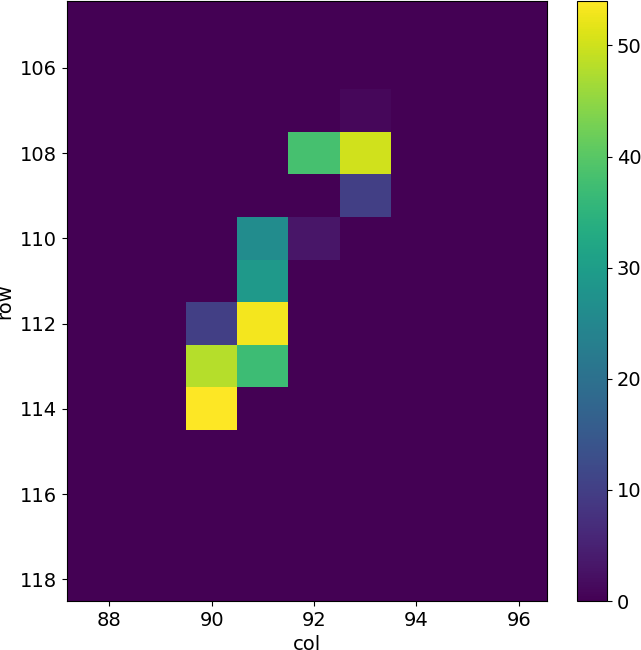
\includegraphics[width=.3\linewidth]{figures/charaterization/evts/cosmic_rays/12.png} 
                    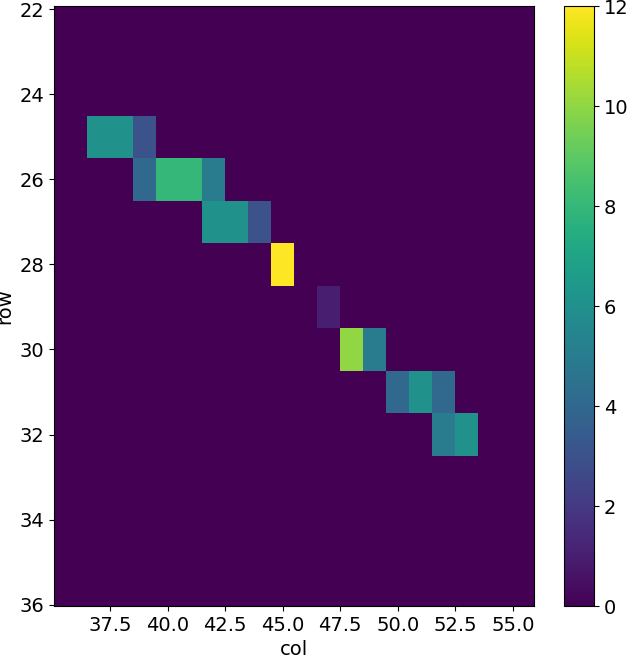
\includegraphics[width=.3\linewidth]{figures/charaterization/evts/cosmic_rays/19a.png}
                \end{figure}
                \begin{itemize}
                    \item Q in cluster is proportional to the cluster size
                    \item MPV $\sim$\SI{500}{\elementarycharge}$^-$
                    \item broad distribution due to the more various sample of particles and energies
                \end{itemize}
        \end{columns}
    \end{frame}    


    %%%%%%%%%%%%%%%%%%%%%%%%%%%%%%%%%%%%%%%%
    %%  Slide 5: <Dead time>  %%
    %%%%%%%%%%%%%%%%%%%%%%%%%%%%%%%%%%%%%%%%
    \begin{frame}
        \frametitle{Readout time}
        \textbf{Injection} allows injecting pulses at different rate. 
        \begin{itemize}
            \item no memory on pixel: 
            \item readout is completely sequential: one serializer @ \SI{40}{MHz}
            \item each hit is a 27-bits data packet, at least \SI{675}{ns} needed
        \end{itemize}

        \medskip
        \begin{columns}
            \column{0.55\textwidth}              
                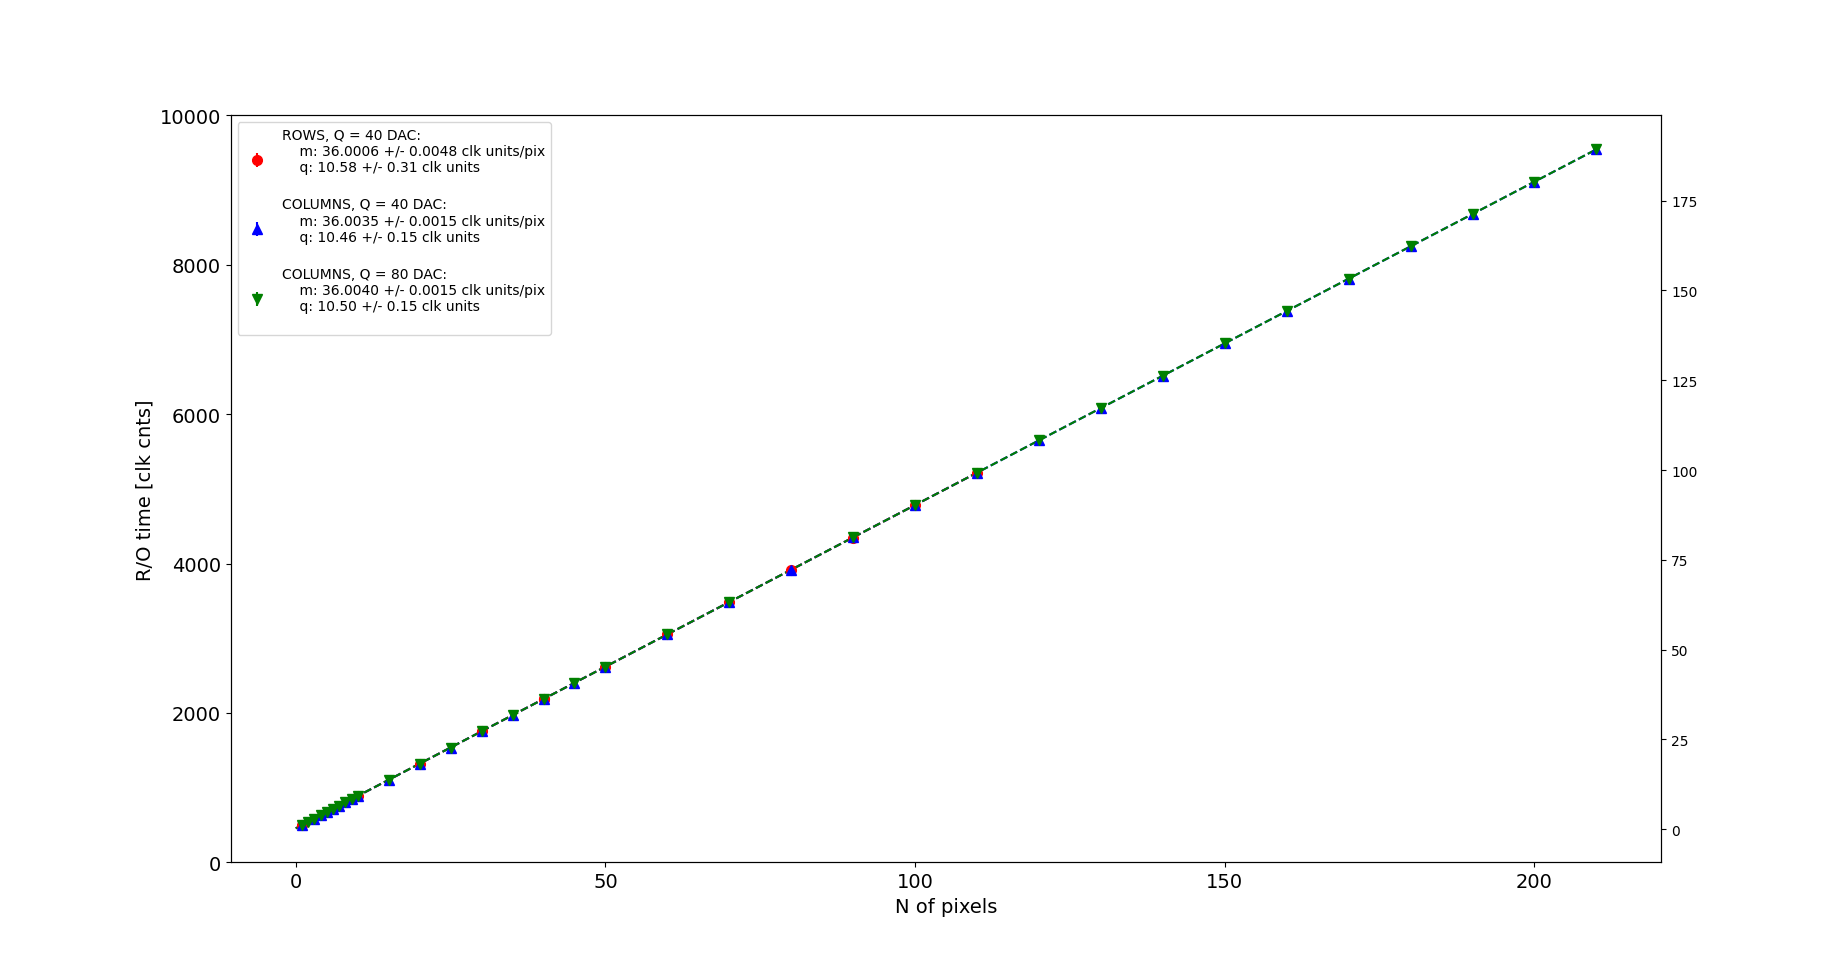
\includegraphics[width=1.07\linewidth]{figures/charaterization/default_line.pdf}
            \column{0.45\textwidth}  
            Readout time \textbf{slightly} depends on the FE status and can be reduced down to \SI{31}{clk.}cnts = \SI{775}{ns} per pixels 

        \end{columns}            
    \end{frame}          